\def\year{2021}\relax
\documentclass[letterpaper]{article} % DO NOT CHANGE THIS
\usepackage{aaai20}  % DO NOT CHANGE THIS
\usepackage{times}  % DO NOT CHANGE THIS
\usepackage{helvet} % DO NOT CHANGE THIS
\usepackage{courier}  % DO NOT CHANGE THIS
\usepackage[hyphens]{url}  % DO NOT CHANGE THIS
\usepackage{graphicx} % DO NOT CHANGE THIS
\urlstyle{rm} % DO NOT CHANGE THIS
\def\UrlFont{\rm}  % DO NOT CHANGE THIS
\usepackage{graphicx}  % DO NOT CHANGE THIS
\frenchspacing  % DO NOT CHANGE THIS
\setlength{\pdfpagewidth}{8.5in}  % DO NOT CHANGE THIS
\setlength{\pdfpageheight}{11in}  % DO NOT CHANGE THIS

\usepackage{amssymb}
\usepackage{amsmath}
% checkmarks
\usepackage{pifont}
\newcommand{\cmark}{\ding{51}}
\newcommand{\xmark}{\ding{55}}


\setcounter{secnumdepth}{2} %May be changed to 1 or 2 if section numbers are desired.



%This is a template for producing LIPIcs articles.
%See lipics-manual.pdf for further information.
%for A4 paper format use option "a4paper", for US-letter use option "letterpaper"
%for british hyphenation rules use option "UKenglish", for american hyphenation rules use option "USenglish"
%for section-numbered lemmas etc., use "numberwithinsect"
%for enabling cleveref support, use "cleveref"
%for enabling cleveref support, use "autoref"


\usepackage{booktabs}
\usepackage[algo2e,vlined]{algorithm2e}

\pdfinfo{
/Title (A* with Fast and Tight Heuristic in Road Networks)
/Author (Ben Strasser, Tim Zeitz)
/Keywords (shortest path, road graphs, goal-directed search, contraction hierarchy, heuristic search)
}
\title{A* with Fast and Tight Heuristic in Road Networks}
\author{Ben Strasser\\
academia@ben-strasser.net\\
\And
Tim Zeitz\\
tim.zeitz@kit.edu\\
Karlsruhe Institute of Technology
}

%%
%% The "author" command and its associated commands are used to define
%% the authors and their affiliations.
%% Of note is the shared affiliation of the first two authors, and the
%% "authornote" and "authornotemark" commands
%% used to denote shared contribution to the research.
%\author{
%Ben Strasser


%\author{Tim Zeitz}
%tim.zeitz@kit.edu}
%\affiliation{%
%  \institution{Institute of Theoretical Informatics, Algorithmics I, Karlsruhe Institute of Technology}
%  \city{Karlsruhe}
%  \country{Germany}
%}


\begin{document}

\maketitle

%%
%% By default, the full list of authors will be used in the page
%% headers. Often, this list is too long, and will overlap
%% other information printed in the page headers. This command allows
%% the author to define a more concise list
%% of authors' names for this purpose.
% \renewcommand{\shortauthors}{Strasser and Zeitz}

%%
%% The abstract is a short summary of the work to be presented in the
%% article.
\begin{abstract}
Efficiently computing flexible and exact routes in continental-sized road networks is a tough challenge.
While Dijkstra's algorithm can be used to solve these problems, it is too slow for many practical applications.
A* is a classical approach to accelerate Dijkstra's algorithm and is used in many fields such as Experimental Algorithms, Robotics, and Artificial Intelligence.
However, A*'s performance depends on the availability of a good heuristic.
Computing a good heuristic is a challenge of its own.
In contrast, for road networks there also exist hierarchical speedup techniques, which do not need a heuristic.
They achieve speed and exactness but sacrifice A*'s flexibility.
In this paper, we use such as Contraction Hierarchies (CH), a hierarchical technique, to compute tight A* heuristics.
We call our technique CH-Potential.
With this approach, we combine some of the speed of hierarchical techniques with the flexibility offered by A* - the best of both worlds - while retaining exactness.
Additionally, we describe A* optimizations to accelerate the processing of low degree nodes, which often occur in road networks.
\end{abstract}

\section{Introduction}
\label{sec:intro}
Route planning in street networks of continental scale is a well-researched topic with many applications~\cite{bdgmpsww-rptn-16}.
It is usually formalized as a variant of the classical shortest path problem in weighted graphs.
Developing flexible techniques to efficiently compute exact routes is a tough challenge.
\emph{Exact} means that the computed path always has minimum weight.
\emph{Efficiently} means that the path computation is fast.
Being able to change the edge weights between path computations or handle more complex edge weights (for example travel times which change over the course of the day obtained through traffic predictions) is \emph{flexibility}.

\begin{figure}

\centering
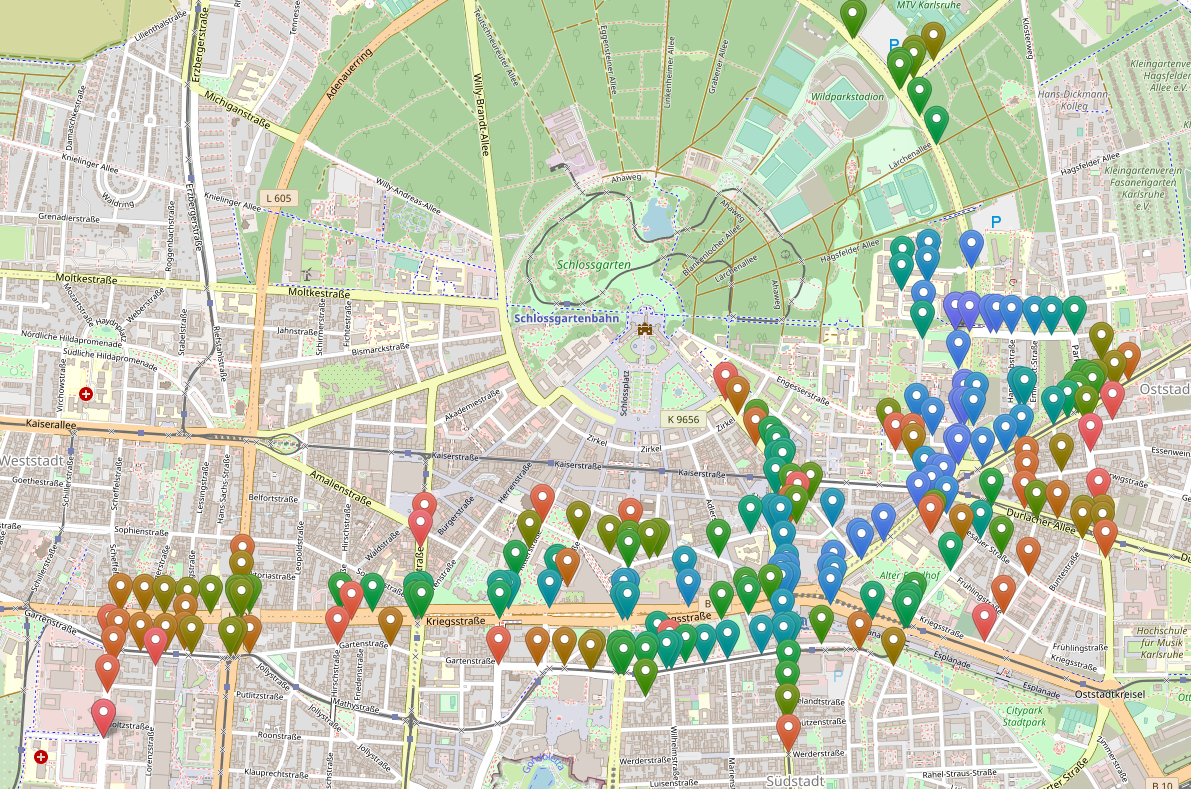
\includegraphics[width=\columnwidth]{fig/searchspace.png}


\caption{Nodes explored by A* with CH-Potentials. Nodes were explored from blue through green to red.}
\label{img:search-space}
\end{figure}


Dijkstra's algorithm~\cite{d-ntpcg-59} achieves flexibility and exactness but is comparatively slow.
Dijkstra's algorithm iteratively explores nodes of the graph with ascending distance from the origin node until the target is reached.
A classic speedup approach is the well-known A* algorithm~\cite{hnr-afbhd-68}.
It changes the order in which nodes are explored by using the distance from the origin plus an estimate of the remaining distance to the target as the ordering criterion.
Figure~\ref{img:search-space} depicts an example A* search.
While flexible, A*'s performance crucially depends on the quality of the employed estimating heuristic.
Finding a good heuristic that can be evaluated efficiently is difficult.

In this paper, we consider a setup with a preprocessing phase and a query phase.
The preprocessing phase can be slow and computes auxiliary data that can be used in the query phase, which should be fast.
The input to the preprocessing phase is the graph weighted with lower bound weights $w_\ell$.
The source/origin $s$ and target/goal $t$ of the path and the actual edge weights $w_q$ are the input to the query phase.
We require that $w_q(e)\ge w_\ell(e)$ for all edges $e$.
In the query phase, the path is computed.
%
Street networks of continental scale have many millions of nodes.
% While the preprocessing phase may be slow, it must eventually finish.
On graphs of this size, quadratic preprocessing time is prohibitive.

In this paper, we consider an algorithm, where the query phase mostly consists of an A* search.
The preprocessing phase computes auxiliary data to efficiently evaluate the heuristic.
Our setup is very similar to the well-known ALT technique~\cite{gh-cspas-05,DBLP:conf/wea/DellingW07}.
We call our algorithm CH-Potentials, as it combines ideas from Contraction Hierarchies (CH)~\cite{gssv-erlrn-12} with A* heuristics, also called potentials in~\cite{gh-cspas-05}.

Formally, a heuristic $h$ is a function that maps nodes onto numbers.
$h$ depends on the target $t$ of the search but not one the source $s$.
Without loss of generality, we assume that $h(t)=0$.
The \emph{tight} heuristic assigns to every node $v$, the length of a shortest $vt$-path.
All heuristics, for which A* is exact, are lower bounds of the tight heuristic.
CH-Potentials compute the tight heuristic with respect to $w_\ell$.
Without access to the query weights $w_q$, which are unavailable during preprocessing, no value of the heuristic can be increased, without loosing A*'s exactness.
In this sense, CH-Potentials are as tight as possible.

\section{Related Work}

A lot of research focuses on the inflexible setting, i.e., the special case where $w_q = w_\ell$.
In this setting, mostly hierarchical approaches dominate in terms of running time~\cite{bdgmpsww-rptn-16}.
A well-known hierarchical technique are Contraction Hierarchies (CH)~\cite{gssv-erlrn-12}.

There is a lot of work that extends CH to handle more complex settings.
For example, in~\cite{fns-opca-14,gks-rpfof-10} multi-criteria optimization is studied.
In~\cite{dsw-cch-15}, CH is modified to support Live-Traffic.
Historic traffic patterns are combined with CH in~\cite{swz-sfert-19,bgsv-mtdtt-13,bdpw-dtdrp-16}.
Specialized variants for electric vehicle routing are developed in~\cite{bdgwz-sfpcs-19}.
While these works show that it is possible to extend hierarchical approaches, they also show that it is non-trivial.
Further, in every setting the flexibility available at query time is fairly limited and usually encompasses only one very specific setting.
Combining all these hierarchical extensions is an unsolved problem.
%
CH-Potentials is not the first work to combine hierarchical approaches and A*~\cite{bdsssw-chgds-10,gkw-blwr-07,bdgwz-sfpcs-19}.
However, past work mostly uses A* to accelerate hierarchical approaches even further and sacrifices A*'s flexibility in the process.
Our primary algorithm design objective is to retain A*'s flexibility.

ALT~\cite{gh-cspas-05} and CPD-Heuristics~\cite{DBLP:conf/ijcai/BonoGHS19} are the two techniques with the highest conceptual similarity to CH-Potentials.
Just as our approach, ALT is A*-based.
However, ALT's heuristic is not tight.
%
CPD-Heuristics are a combination of A* and Compressed Path Databases (CPD).
A CPD can quickly compute the first edge of a shortest path between any two nodes.
In~\cite{DBLP:conf/ijcai/BonoGHS19}, SRC~\cite{DBLP:conf/socs/StrasserHB14} is used as CPD.
For every distance estimation, a shortest path to the target is computed, whose length is used as the tight heuristic.
Unfortunately, the CPD used has quadratic preprocessing running times, which is prohibitively expensive on large street networks.
%
MtsCopa~\cite{DBLP:journals/tciaig/BaierBHH15} uses a similar idea to CPD-Heuristics but is only applied in a hunter-prey application.
%
In~\cite{DBLP:conf/ijcai/0002UJAKK18} the weighted graph is embedded into Euclidean space using FastMap such that distances in space and distances in the graph roughly correspond.
The Euclidean distance is then used as A* heuristic.
%
The handling of low degree nodes in our A* search is a variation of the techniques used in TopoCore~\cite{DBLP:conf/gis/DibbeltSW15}, which is inspired by~\cite{DBLP:journals/pvldb/FunkeNS14}.

\subsection{Oracle-A* \& Comparison with Related Work}

To compare against related work, we introduce the concept of Oracle-A*.
It has access to a shortest distance array with respect to $w_\ell$, i.e., it is tight.
This is the tightest potential achievable during preprocessing.
The array computation time is unaccounted for, i.e., it is magically filled instantly.
Oracle-A* is not achievable in practice.
However, it is a lower bound for every algorithm following our setup.
We experimentally show that CH-Potentials are within a factor two of Oracle-A* and thus every related work.

\subsection{Applications need Flexibility}

Many applications need flexibility.
The most common ones are traffic avoidance, user preferences, and vehicle restrictions.
Traffic avoidance comes in two forms: Live~\cite{dgpw-crprn-13,dsw-cch-15} and predicted traffic~\cite{ndls-bastd-12,bgsv-mtdtt-13}.
Predicted traffic is often called time-dependent routing.
%
User preferences can vary significantly~\cite{DBLP:conf/gis/FunkeS15,DBLP:conf/gis/DellingGGKTW15,DBLP:conf/gis/FunkeLS16}.
For example, for some users shorter routes are more important than fast routes.
Others want to avoid tunnels or highways.
%
Truck routing differs from car routing due to night driving bans and other restrictions~\cite{kswz-erptd-20}.
%
Flexibility is also often used as building block in multi-agent planning settings~\cite{DBLP:journals/ai/SharonSFS15,DBLP:journals/tciaig/BaierBHH15}.
%
Electric Vehicle Routing also requires flexibility~\cite{DBLP:journals/algorithmica/BaumDPSWZ20,DBLP:conf/aaai/EisnerFS11}.

\section{Contribution \& Outline}

We introduce CH-Potentials, a two-phase technique to efficiently compute tight heuristics, in Section~\ref{sec:main-algo}.
Combined with A*, this yields an exact, efficient, and flexible route planning algorithm.
Beside the heuristic, in Section\ref{sec:low-deg-improvment}, we describe some improvements to A* to more efficiently process low degree nodes, common in road networks.
In Section~\ref{sec:extensions}, we demonstrate CH-Potential's flexibility, by describing various extended route planning applications and how they can be solved using CH-Potentials.
Finally, in Section~\ref{sec:experiments}, we present an experimental evaluation of our approach.
By comparing against Oracle-A*, we show that no alternative approach can be significantly faster, assuming that $w_\ell$ is the tightest lower bound that can be known in advance.

\section{Algorithm Description}

In this section, we first describe Contraction Hierarchies, then PHAST, and finally CH-Potentials.

\label{sec:main-algo}

\begin{algorithm2e}
\KwData{$B[x]$: tentative distance from $x$ to target $t$}
\KwData{Min. priority queue $Q$, also called open list}
$B[x] \leftarrow +\infty$ for all $x\neq t$;
$B[t] \leftarrow 0$\;
Make $Q$ only contain $t$ with weight $0$\;
\While{not $Q$ empty}{
	$y\leftarrow$ pop minimum element from $Q$\;
	\For{$xy$ is down-edge in $G^+$}{
		\If{$B[x] > w_\ell(xy) + B[y]$}{
			$B[x]\leftarrow w_\ell(xy) + B[y]$\;
                        Add $x$ or decrease $x$'s key in $Q$ to $B[x]$\;
		}
	}
}
\caption{CH backward search}
\label{algo:ch-backward}
\end{algorithm2e}

\begin{figure}
\centering
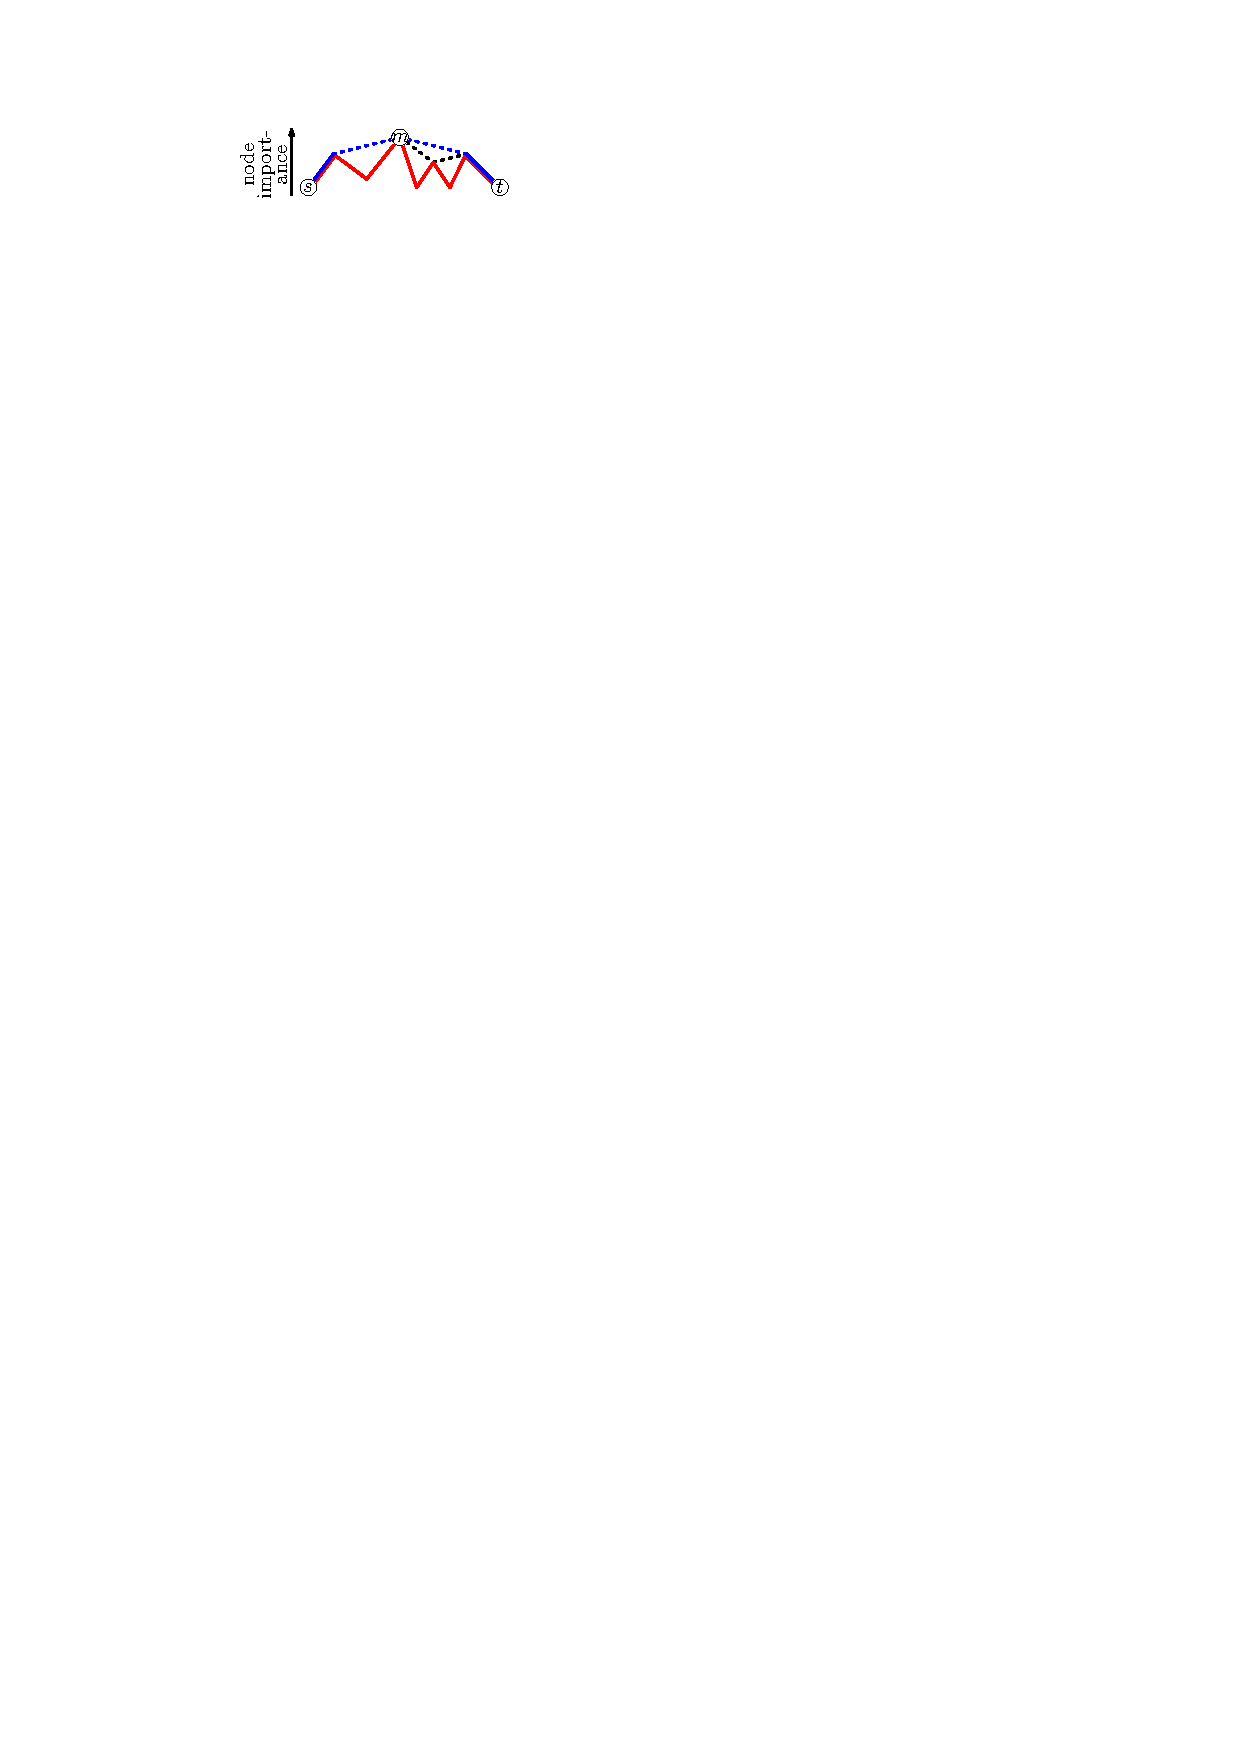
\includegraphics{fig/ch}
\caption{
Solid lines are edges in $G$. Dotted lines are shortcuts. Red is shortest $st$-path in $G$. Blue is equaly long up-down $st$-path in $G^+$. $m$ is mid node.
}
\label{fig:ch}
\end{figure}

\subsection{Contraction Hierarchy (CH)}

A CH is a two phase technique to efficiently compute exact, shortest paths.
It is not flexibile, i.e., $w_q=w_\ell$.
For a details, we refer the interested reader to \cite{gssv-erlrn-12,dsw-cch-15}.
In this section, we give an introduction.

A CH places nodes into levels.
No edge must connect two nodes within one level.
Levels are ordered by ``importance''.
The intuition is that dead-ends are unimportant and at the bottom while highway bridges are very important and at the top.
An edge goes \emph{up} when it goes from a node in a lower level to higher level.
\emph{Down} edges are defined analogously.
An \emph{up-down path} is a path where only one node $v$ is more important than both its neighbors.
$v$ is called the \emph{mid} node.
An \emph{up path} is a path where the last node is the mid node.
Similarly, the first node is the mid node of a \emph{down path}.
Every up and down path is an up-down path.
%
In the preprocessing phase, a CH adds \emph{shortcut} edges to the input graph $G$ to obtain $G^+$.
This is done by repeatedly contracting unimportant nodes and adding shortcuts between its neighbors.
See~\cite{gssv-erlrn-12} for the details.
After the preprocessing, in $G^+$ for pair of nodes $s$ and $t$ there exists a shortest up-down $st$-path with the same length as a shortest path in $G$.
See Figure~\ref{fig:ch} for a proof sketch.
From every shortest path (red) in $G$, a up-down path of equal length in $G+$ (blue) can be constructed.
We may therefore restrict our search to up-down paths in $G^+$.
This search is bidirectional.
The forward search starts from $s$ and only follows up-edges.
Similarly, the backward search starts at $t$ and only follows down-edges in reversed direction.
The two searches meet at the mid node.
Pseudo-code for the backward search, i.e., the path from $m$ to $t$, is presented in Algorithm~\ref{algo:ch-backward}.
The forward search works analogously.
%
A CH query is fast, if the number of nodes reachable via only up- or down-nodes is small.
On road networks, this is the case as demonstrated in~\cite{gssv-erlrn-12,dgrw-gpnc-11,dgpw-crprn-13,dsw-cch-15,hs-gbpo-18}.

Using a CH, we can compute a tight A* heuristic.
In the preprocessing phase, a CH with respect to $w_\ell$ is computed.
The query phase consists of an A* search, where the evaluation of the heuristic $\pi(v)$ performs a CH-query from $v$ to $t$.
%
This works, however, while one CH query is fast, answering one for every node explored in the $A^*$ search is slow.
Fortunately, we can do better.
However, for this we need another component called PHAST~\cite{dgnw-phast-13}.

\subsection{Potentials using PHAST}

\begin{algorithm2e}
\KwData{$P[x]$: tentative distance from $x$ to $t$}
Execute Algorithm~\ref{algo:ch-backward}\;
\For{all CH levels $L$ from most to least important}{
	\For{all up edges $xy$ in $G^+$ with $x$ in $L$}{
		\If{$P[x] < P[y] + w_\ell(xy)$}{
			$P[x] \leftarrow P[y] + w_\ell(xy)$\;
		}
	}
}
\caption{PHAST basic all-to-one search}
\label{algo:phast}
\end{algorithm2e}

PHAST~\cite{dgnw-phast-13} is a CH extension that computes distances from all nodes to one target node.
First the preprocessing phase is executed analogously to the original CH.
The query phase is divided into two steps.
The first step is analogously to the CH query:
From the target node $t$, all reachable nodes via reversed down-edges are explored.
Algorithm~\ref{algo:ch-backward} shows this first step.
The second step iterates over all CH levels from top to bottom.
In each iteration, all up-edges starting within the current level are followed in reverse.
After all levels are processed, the distances from all nodes towards $t$ is computed.
PHAST is slightly faster than Dijkstra's algorithm on road graphs because it is a better fit for modern processor architectures.
PHAST's main advantage is that can easily be parallelized.
However, we will not consider parallelization in this paper.
We refer to~\cite{dgnw-phast-13} for an in-depth experimental performance analysis.
Pseudo-code is provided in Algorithm~\ref{algo:phast}.
Using PHAST, we can compute a tight A* heuristic in another way.
In the query phase, we first use PHAST to compute the distances from every node to $t$ with respect to the query edge weights $w_\ell$ and store the result in an array $H$.
In the next step, we run $A^*$ and implement the heuristic function as lookup in the array $H$.

This PHAST-based algorithm works.
The heuristic evaluation and by extension the $A^*$ search is indeed fast.
However, the PHAST step before the search is comparatively expensive.
The reason for this is that the distances from all nodes towards $t$ are computed.
Ideally, we only want to compute the distances from the nodes explored in the $A^*$ search towards $t$.

\subsection{CH-Potentials}

\begin{algorithm2e}
\KwData{$B[x]$: tentative distance from $x$ to $t$ as computed by Algorithm~\ref{algo:ch-backward}}
\KwData{$P[x]$: memoized potential at $x$, $\bot$ initially}
\SetKwFunction{Pot}{Pot}
\SetKwProg{Fn}{Function}{:}{}
\Fn{\Pot{$x$}}{
	\If{$P[x] = \bot$}{
		$P[x]\leftarrow B[x]$\;
		\For{all up edges $xy$ in $G^+$}{
                        $P[x]\leftarrow\min\{P[x],w_\ell(xy)+\Pot(y)\}$\;
		}
	}
	\Return{$P[x]$}\;
}
\caption{CH-Potentials Algorithm}
\label{algo:pot}
\end{algorithm2e}

Fortunately, the PHAST computation can be done lazily using memoization as depicted in Algorithm~\ref{algo:pot}.
In a first step, we run the backward CH search from $t$ to obtain an array $B$.
$B[v]$ is the minimum down $vt$-path distance or $+\infty$, if there is no such path.
$B$ is computed as shown in Algorithm~\ref{algo:ch-backward}.

Suppose, we need to compute the potential $\pi(v)$ of a node $v$.
We do this by first recursively computing the potentials $\pi(u)$ of all nodes for which an up-edge $(v,u)$ exists.
Afterwards, we compute using $\min_u\{w_\ell(v,u) + \pi(u)\}$ the minimum distance over all up-down paths that contain at least one up-edge.
As the minimum distance up-down path does not necessarily have to contain an up-edge, we set $\pi(v) = \min \{ B[v], \min_u\{w_\ell(v,u) + \pi(u)\} \}$.
This calculation is correct, as it computes the minimum up-down $vt$-path distance in $G^+$, which corresponds to the minimum $vt$-path distance in a CH.

The resulting algorithm is the basic CH-potential algorithm.
It is flexible and exact.
However, we can still improve the performance.
A quick investigation reveals, that a significant amount of running time is spent in the heuristic evaluation.
We therefore investigate methods to evaluate the heuristic less often.

\section{Low Degree A* Improvements}

\label{sec:low-deg-improvment}

Heuristic evaluation is an expensive operation that we want to avoid.
The heuristic needs to be evaluated when a node is pushed into the queue.
By avoiding push operations, we can therefore avoid heuristic evaluations.
This is the objective of this section.

\subsection{Skip Degree Two Nodes}

We modify A* by processing low degree nodes consecutively without pushing them into the queue.
Our algorithm makes use of the undirected degree $d(x)$ of a node $x$.
Formally, $d(x)$ is the number of nodes $y$ such that $(x,y)\in E$ or $(y,x)\in E$.

Analogous to A*, our algorithm stores for every node $x$ a tentative distance $D[x]$.
Additionally, it maintains a minimum priority queue.
Diverging from A*, not all nodes can be pushed but every node has a tentative distance.

Our algorithm differs from A* when removing a node $x$ from the queue.
A* iterates over the outgoing arcs $(x,y)$ of $x$ and tries to reduce $D[y]$ by relaxing $(x,y)$.
If A* succeeds, $y$'s weight in the queue is set to $D[y]+\pi(y)$.
Our algorithm, however, behaves differently, if $d(y)\le 2$.
Our algorithm determines the longest degree two chain of nodes $x,y_1,\ldots, y_k, z$ such that $d(y_i)=2$ and $d(z) > 2$.
If our algorithm succeeds in reducing $D[y_1]$, it does not push $y_1$ into the queue.
Instead, it iteratively tries to reduce all $D[y_i]$.
If it does not reach $z$, then only $D$ is modified but no queue action is performed.
If $D[z]$ is modified and $d(z)>2$, $z$'s weight in the queue is set to $D[z]+\pi(z)$.

As the target node $t$ might have degree two, our algorithm cannot rely on stopping, when $t$ is removed from the queue.
Instead, our algorithm stops as soon as $D[t]$ is less than the minimum weight in the queue.

\subsection{Skip Degree Three Nodes}

In the previous section, we described an optimized A* variant that does not push degree two nodes.
In this section, we also avoid degree three nodes.

Denote by $x,y_1,\ldots, y_k, z$ a degree two chain as described in the previous section.
If $d(z) > 3$ or $z$ is in the queue, our algorithm proceeds as in the previous section.
Otherwise, there exist up to two degree chains $z,a_1,\ldots,a_p,b$ and $z,\alpha_1,\ldots,\alpha_q,\beta$ such that $a_1\neq y_k \neq \alpha_1$.
Our algorithm iteratively tries to reduce all $D[a_i]$ and $D[\alpha_i]$.
If it reaches $\beta$, $\beta$'s weight in the queue is set to $D[\beta]+\pi(\beta)$.
Analogously, if $b$ is reached, $b$'s weight is set to $D[b]+\pi(b)$.
If $b$ respectively $\beta$ are not reached, our algorithm does nothing.

\subsection{Stay in Largest Biconnected Component}

\label{sec:largested-biconnected-component}

A lot of nodes in road networks lead to dead-ends.
Unless the source or target is is in a dead-end, it is unnecessary to explore these nodes.
This reduces the number of explored nodes and thus leads to fewer heuristic evaluations.

In the preprocessing phase, before the CH is created, we compute the subgraph $G_C$, called \emph{core}, induced by the largested biconnected component of the undirected graph underlying $G$.
We do this using Tarjan's algorithm \cite{t-dfslg2-72}.
For every node $v$ in the input graph $G$, we store the attachment node $a_v$ to the core.
For nodes in the core, $a_v=v$.
We exploit that all attachment nodes are single node separators and the problem can be decomposed along them.
The CH-Potentials preprocessing step is only executed for $G_C$.

The query phase is divided into four steps.
In the first step, we use Dijkstra's algorithm to explore the component that contains $s$ until $a_s$ is reached.
If this search finds $t$, then $s$ and $t$ are part of the same component.
A shortest path was found and therefore the algorithm stops early.
Otherwise, in the second step starts.
It consists of applying the CH-Potential algorithm restricted to $G_C$ from $a_s$ to $a_t$.
Finally, in the third step, we search a path from $a_t$ towards $t$ using Dijkstra's algorithm restricted to $t$'s biconnected component.
The final path is the concatenation of all three path parts.

\section{Algorithm Extensions}
\label{sec:extensions}

A* is a very flexible algorithm.
Many extended problems can therefore be solved using the CH-Potentials algorithm.
In this section, we describe some extended problems.

\subsection{Avoiding Tunnels and/or Highways}
\label{sec:no-tunnel-highway}

Avoiding tunnels and/or highways is a common feature of navigation devices.
Implementing this feature with CH-Potentials is easy.
We set $w_\ell$ to the freeflow travel time.
If an edge is a tunnel and/or a highway, we set $w_q$ to $+\infty$.
Otherwise, $w_q$ is set to the freeflow travel time.
This is all that is necessary to make our CH-Potentials algorithm avoid tunnels and/or highways.

\subsection{Forbidden Turns and Turn Costs}
\label{sec:no-turns}

The classical shortest path problem allows to turn from every edge to every other incident edge at every node.
However in the real world, turn restrictions, such as a forbidden left or right turn, exist.
Such restrictions are usually modeled using turn weights.
We extend CH-Potentials by using zero as lower bound for every turn weight in the heuristic.
In this section, we first present the extended problem setting.
Afterwards, we describe how it can be solved with CH-Potentials.

In the extended problem, a \emph{turn weight} $w_t$ is introduced~\cite{gv-errnt-11,dgpw-crprn-13,bwzz-cchtc-20}.
$w_t$ maps a pair of incident edges onto the time required to perform the turn.
Formally, $w_t$ is a function from $V^3$ to $\mathbb{R}^+ \cup \{+\infty\}$.
A forbidden turn is modeled by setting the corresponding $w_t$ to $+\infty$.

A path with nodes $v_1, v_2,\ldots v_k$ has the following \emph{turn-aware path weight}:\[
w_q(v_1, v_2) + \sum_{i=2}^{k-1}  w_t(v_{i-1},v_i,v_{i+1})  + w_q(v_i,v_{i+1})
\] The input to the extended problem consists of a source edge and a target edge.
The objective is to find a path connecting these edges such that the turn-aware path weight is minimized.
The first term $w_q(v_1, v_2)$ only depends on the source edge.
As all considered paths share the same source edge, the term is the same for all paths.
We can therefore ignore it during the optimization.

To account for turns, many algorithms construct a \emph{turn-expanded} graph $G'$.
Edges in the input graph $G$ correspond to \emph{expanded nodes} in $G'$.
For every pair of successive edges $(x,y)$ and $(y,z)$ in $G$, there is an \emph{expanded edge} in $G'$ with expanded weight $w_t(x,y,z) + w_q(y,z)$.
A sequence of expanded nodes in the expanded graph $G'$ corresponds to a sequence of edges in the input graph $G$.
The weight of a path in $G'$ is equal to the turn-aware weight of the corresponding path in $G$ minus the irrelevant $w_q(v_1,v_2)$ term.
Turn-aware shortest paths can thus be computed by searching for shortest paths in the expanded graph.

The simplest combination of turn-aware routing with CH-Potentials consists of using the expanded graph as input to the CH-Potential algorithm.
However, this implies computing a CH on the expanded graph.
This is feasible but has a number of problems such as higher preprocessing running time, increased memory consumption, or more complex code~\cite{gv-errnt-11}.
We want to avoid these complications.

We therefore only apply the A* search to the expanded graph $G'$.
The heuristic is computed with respect to the input graph $G$.
Let $(p,q)$ be the target edge and $(x,y)$ the edge for which the A* search wants to compute a heuristic.
We construct non-turn-aware CH-Potentials towards $q$.
The heuristic for the edge $(x,y)$ is equal to the heuristic of $y$.

To prove correctness, consider the turn-aware path weight of a shortest path $v_1,v_2\ldots v_k$ with $v_1=x$, $v_2=y$, $v_{k-1}=p$, and $v_k=q$.
We can lower bound the expression as follows:
\[
\sum_{i=2}^{k-1} w_\ell(v_i,v_{i+1}) \le \sum_{i=2}^{k-1} \underbrace{w_t(v_{i-1},v_i,v_{i+1})}_{0\le} + \sum_{i=2}^{k-1} \underbrace{w_q(v_i,v_{i+1})}_{w_\ell(v_i,v_{i+1})\le}
\]
The $\sum_{i=2}^{k-1} w_\ell(v_i,v_{i+1})$ expression is the length of some, not necessarily shortest, $yq$-path in $G$ with $w_\ell$.
It is by definition not smaller than the shortest $yq$-path length in $G$ with $w_\ell$.
The shortest $yq$-path length is exactly what CH-Potentials compute.
The heuristic is therefore a lower bound.
It is consistent because it is derived from exact shortest paths in $G$ with $w_\ell$.

Unfortunately, the undirected graph underlying the expanded graph is always biconnected, if the input graph is strongly connected.
The optimization described in~\ref{sec:largested-biconnected-component} is therefore ineffective in this setting.

With this setup we extend CH-Potentials in a way that keeps all turn-related information out of the CH.
This allows for a comparatively simple implementation.

\subsection{Predicted Traffic or Time-Dependent Routing}
\label{sec:predicted-traffic}

The classical shortest path problem assumes that edge weights are scalars.
However in practice, travel times vary along an edge.
The primary reason is traffic.
Recurring traffic can be predicted by observing the traffic in the past.
It is common \cite{bgsv-mtdtt-13,bdpw-dtdrp-16,swz-sfert-19} to represent these predictions as \emph{travel time functions}.
An edge weight is no longer a scalar value but a function that maps the entry time onto the traversal time.
Performing this prediction is outside of the scope of this paper.
It is common to refer to routing with predicted traffic as \emph{time-dependent routing}.
Again, we first formalize the extended problem setting and then describe our solution with CH-Potentials.

Formally, $w_q$ is a function from $E\times \mathbb{R}$ to $\mathbb{R}^+$.
$w_q(e, \tau)$ is the travel time through edge $e$ when entering it at moment $\tau$.
The input to the extended problem consists of a source node $s$ and a target node $t$, as in the classical problem formulation.
Additionally, the input contains a source time $\tau_s$.
A path with edges $e_1,e_2\ldots e_k$ is weighted using $\alpha_k$, which is defined recursively as follows:\[
\begin{split}
\alpha_{1} & = w_q(e_1, \tau_s) \\
\alpha_{k} & = \alpha_{k-1} + w_q(e_1, \alpha_{k-1})
\end{split}
\]
The objective is to find a path that minimizes $\alpha_k$.

If all travel time functions fulfill the \emph{no-waiting property}, this problem can be solved using a straight forward extension of Dijkstra's algorithm \cite{d-aassp-69}.
The necessary modification to A* is analogous.
Without the no-waiting property the problem is in general NP-hard \cite{or-tnp-89}.
The no-waiting property states that it is never beneficial to wait at a node before entering an edge.
Formally stated, the following must hold:\[
\forall e\in E,\tau\in \mathbb{R},\delta\in \mathbb{R}^+: w_q(e, \tau) \le w_q(e, \tau+\delta) + \delta
\]

Usually, travel time functions are stored as piece-wise linear functions.
Our implementation follows this setup.
However in principle, our algorithm works with any representation that enables an efficient function evaluation.

To solve the time-dependent routing problem, we employ a strategy very similar to TD-ALT~\cite{ndls-bastd-12}.
The main difference is that we use CH-Potentials instead of landmarks to guide the A* search.
We set $w_\ell(e)$ to the minimum travel time for every edge, i.e., $w_\ell(e) = \min_\tau w_q(e,\tau)$.

We modify the A* search to use the tentative distance at a node $x$ as $\tau$ when evaluating the weight of an outgoing edge $(x,y)$.
This modification is straight-forward, as our optimizations do not use shortcuts and only traverse edges in forward direction.
For the correctness proof, we refer to~\cite{dw-lbrdg-07}.

With this setup, we extended CH-Potentials to support time-dependent routing.
As we were able to keep all travel time functions out of the CH.
This avoids a lot of algorithmic complications compared to~\cite{bgsv-mtdtt-13,bdpw-dtdrp-16,swz-sfert-19}, which create shortcuts of travel time functions to combine hierarchical speedup techniques with time-dependent routing.

\subsection{Live and Predicted Traffic}
\label{sec:live-predicted-traffic}

Beside predicted traffic, we also consider live traffic.
Live traffic refers to the current traffic situation.
It is important to distinguish between predicted and live traffic.
The predicted travel time along an edge was estimated in the past.
It is possible that it differs from the current travel time significantly, if unexpected events happen.
Accidents are examples of such unexpected events.
Live traffic data is more accurate for the current moment than predicted data.
However, just using live traffic data is problematic for long routes as traffic changes while driving.
At some point, one wants to switch from live traffic back to the predicted traffic.
In this section, we first describe how to use only live traffic and then describe how to combine it with predicted traffic.

To support live traffic, we set $w_\ell$ to the travel time without any congestions.
$w_q$ is set to the travel time accounting for the current traffic.
As traffic only increases the travel time along an edge, $w_\ell$ is a valid lower bound for $w_q$.
With this setup, the CH-Potentials algorithms can make use of live traffic.

To combine live traffic with predicted traffic, we define a modified travel time function.
Denote by $w_p(e,\tau)$ the predicted travel time along edge $e$ at moment $\tau$.
Further, $w_c(e)$ is the travel time according to the live traffic.
Finally, we denote by $\tau_{\mathrm{soon}}$ the moment up to which we trust the live traffic.
In our experiments, we set $\tau_{\mathrm{soon}}$ to one hour in the future.
We need to make sure that the modified travel time function fulfills the no-waiting property.
For this reason, we cannot make a hard switch at $\tau_{\mathrm{soon}}$.
Our modified travel time function linearly approaches the predicted travel time with a bounded slope.

Formally, we set $w_q(e,\tau)$ to $w_c(e)$, if $\tau \leq \tau_{\mathrm{soon}}$.
Otherwise, we check whether $w_p(e,\tau_{\mathrm{soon}}) < w_c(e)$ is true.
If it is the case, we set $w_q(e,\tau)$ to $\max\{w_c(e)+(\tau_{\mathrm{soon}}-\tau), w_p(e,\tau)\}$.
Otherwise, we set $w_q(e,\tau)$ to $\min\{w_c(e)-(\tau_{\mathrm{soon}}-\tau), w_p(e,\tau)\}$.
We set $w_\ell$ again to the freeflow travel time.
Finally, we run the modified time-dependent A* described in the previous section on this modified travel time function.
In our implementation, we to not modify the representation of $w_p$.
Instead, we evaluate the formulas above each time that the modified travel time function is evaluated.

With this setup, we extended CH-Potentials to support a combination of live and predicted traffic.
We did not make any modification to our algorithm, that would make a combination with tunnel and/or highway avoidance or turn-aware routing difficult.
This straight-forward integration of complex routing problems is the strength of the CH-Potential algorithm.

\section{Evaluation}

\label{sec:experiments}

\begin{table}
\centering
\caption{Instances used in the evaluation.}\label{tab:graphs}
\begin{tabular}{lrrrrr}
\toprule
 &                &                & \multicolumn{3}{c}{Preprocessing [s]} \\ \cmidrule(lr){4-6} & Nodes          & Edges          & \multirow{2}{*}{CH} & \multicolumn{2}{c}{CCH} \\ \cmidrule(lr){5-6} & $[\cdot 10^6]$ & $[\cdot 10^6]$ &                     & Phase 1 & Phase 2 \\
\midrule
OSM Germany   &       16.2 &       35.4 &                          298.7 &        1\,467.4 &          10.1 \\
DIMACS Europe &       18.0 &       42.2 &                          276.2 &        2\,480.9 &          12.4 \\
TDGer06       &        4.7 &       10.8 &                           59.2 &         331.7 &           2.7 \\
TDEur17       &       25.8 &       55.5 &                          293.9 &        2\,102.3 &          14.1 \\
TDEur20       &       28.5 &       60.9 &                          311.9 &        2\,219.5 &          15.2 \\
\bottomrule
\end{tabular}


\end{table}

\begin{figure*}
\centering
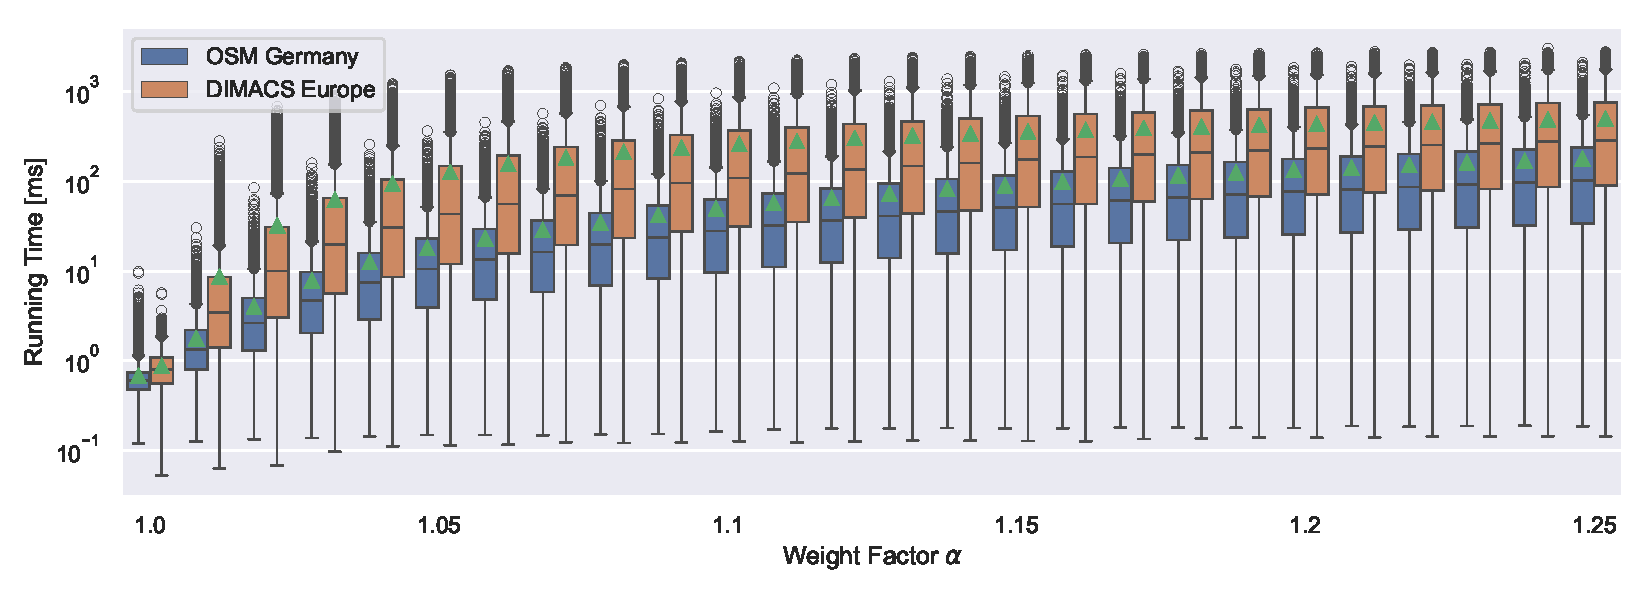
\includegraphics[width=\textwidth]{fig/scaled_weights.pdf}
\caption{
Running times on a logarithmic scale for queries on OSM Ger with scaled edge weights $w_q = \alpha \cdot w_\ell$.
The boxes cover the range between the first and third quartile.
The band in the box indicates the median, the diamond the mean.
The whiskers cover 1.5 times the inter quartile range.
All other running times are marked as outliers.
}\label{fig:scaled_weights}
\end{figure*}

In this section, we present our experimental evaluation.
Our benchmark machine runs openSUSE Leap 15.1 (kernel 4.12.14), and has 128\,GiB of DDR4-2133 RAM and an Intel Xeon E5-1630 v3 CPUs which has four cores clocked at 3.7\,Ghz and 4~$\times$~32\,KiB of L1, 8~$\times$~256\,KiB of L2, and 10\,MiB of shared L3 cache.
All experiments were performed sequentially.
Our code is written in Rust and compiled with rustc 1.47.0-nightly in the release profile with the target-cpu=native option.

\subparagraph{Inputs and Methodology}
Our main benchmark instance is a graph of the road network of Germany obtained from Open Street Map\footnote{\url{https://download.geofabrik.de/europe/germany-200101.osm.pbf}}.
To obtain the routing graph, we use the import from RoutingKit\footnote{\url{https://github.com/RoutingKit/RoutingKit}}.
The graph has 16M nodes and 35M edges.
For this instance, we have proprietary traffic data provided by Mapbox\footnote{\url{https://www.mapbox.com/}}.
The  data includes a live traffic snapshot from Friday 2019/08/02 afternoon and comes in the form of 320K OSM node pairs and live speeds for the link between the nodes.
It also includes traffic predictions for 38\% of the links as predicted speeds for all five minute periods over the course of a week.
Additionally, have two graphs with traffic predictions provided by PTV\footnote{\url{https://ptvgroup.com}}.
One is an old instance of Germany with traffic predictions from 2006 (4.7M nodes, 10.7M edges) and the other a newer instance of Europe (25.8M nodes, 55.5M edges, from 2017).
Table~\ref{tab:graphs} contains an overview over our instances.
We report preprocessing running times as averages over 10 runs.
For the queries, we perform 10\,000 point-to-point queries where both source and target are nodes drawn uniformly at random and report average results.

\subparagraph{Experiments}
We first investigate the effectiveness of the heuristic depending on how tight the lower bound is.
For that, we take our main graph, use the unmodified travel time metric as the lower bound $w_\ell$, and perform queries on $w_q = \alpha \cdot w_\ell$ where $\alpha$ is a factor $\geq 1$.
When $\alpha = 1$, the heuristic is as tight as possible.
With growing $\alpha$ the heuristic degrades.
Figure~\ref{fig:scaled_weights} depicts the results.
Clearly, $\alpha$ has significant influence on the running time.
Average running times range from below a millisecond to a few hundred milliseconds depending on $\alpha$.
Up to around $\alpha = 1.1$ the running time growth is roughly quadratic before leveling off to something more resembling linear growth.
We observe a significant amount of heavy outliers sometimes more than an order of magnitude slower than the median.
Generally, running times vary quite strongly even though most queries are long range queries as we draw source and target node uniformly at random.
The reason is that different queries (even with similar shortest path lengths) are affected differently by growing $\alpha$ depending on the geographic regions the shortest path traverses.
When $\alpha$ grows, more and more nodes in the area around the shortest paths are explored.
So when the shortest path traverses an area where many nodes are reachable in short distance, the search space grows stronger, than when the shortest path goes only through sparse areas.
% Conclusions?

\begin{table}
\centering
\caption{Query performance with different heuristics and optimizations on OSM Ger with $w_q = 1.05 \cdot w_\ell$.}\label{tab:building_blocks}
\begin{tabular}{clllrrrrr}
\toprule
       & BCC & Deg2 & Deg3 & Zero & ALT & CH & CCH & Oracle \\
\midrule
\multirow{4}{*}{\rotatebox[origin=c]{90}{\shortstack{Running\\time [ms]}}} & \xmark &        \xmark &        \xmark &  2\,133.0 &  317.9 &   47.9 &   54.4 &    34.3 \\
                                                                                    & \cmark &        \xmark &        \xmark &  1\,355.3 &  233.9 &   36.3 &   38.5 &    24.8 \\
                                                                                    & \cmark &         \cmark &        \xmark &   753.4 &  122.6 &   19.5 &   22.1 &    12.7 \\
                                                                                    & \cmark &         \cmark &         \cmark &   580.7 &   90.8 &   15.9 &   18.1 &    10.1 \\
\addlinespace
\multirow{4}{*}{\rotatebox[origin=c]{90}{\shortstack{Queue\\pushs[$\cdot 10^3$]}}} & \xmark &        \xmark &        \xmark &  8\,087.1 &  863.1 &  137.1 &  137.1 &   137.1 \\
                                                                                    & \cmark &        \xmark &        \xmark &  6\,298.2 &  685.7 &  112.7 &  112.7 &   112.7 \\
                                                                                    & \cmark &         \cmark &        \xmark &  2\,901.4 &  303.4 &   43.3 &   43.3 &    43.3 \\
                                                                                    & \cmark &         \cmark &         \cmark &  1\,681.4 &  179.7 &   26.8 &   26.8 &    26.8 \\
\bottomrule
\end{tabular}


\end{table}

In Table~\ref{tab:building_blocks} we investigate the impact of our optimizations.
We run queries with different heuristic functions: the \emph{Zero} heuristic which turns A* back into the classical algorithm of Dijkstra, our new CH-Potential heuristic, and an \emph{Oracle} heuristic where all distances to $t$ with regards to $w_\ell$ can be obtained immediately.
We first observe that each one of our optimizations gains useful speedups regardless of the heuristic used.
Our optimizations do not only reduce heuristic evaluations but also queue operations which always accelerates the algorithm.
The number of queue pushs roughly corresponds to the running time for all heuristics.
When comparing CH-Potentials to the Oracle heuristic we note that CH-Potentials are only a factor of 1.6 slower.
This clearly shows that CH-Potentials have very little overhead.
Assuming that $w_\ell$ is the tightest possible lower bound that can be known in advance, no other heuristic can be more than a factor of 1.6 faster than CH-Potentials without sacrificing exactness.

\begin{table*}
\centering
\caption{
CH-Potentials performance for different route planning applications.
We report average running times and number of queue pushs.
We also report the average length increase, that is how much longer the final shortest distance is compared to the lower bound.
Finally, we report the average running time of Dijkstras algorithm as a baseline and the speedup of CH-Potentials over the baseline.
}\label{tab:applications}
\begin{tabular}{llrrrrrr}
\toprule
 & & &   Running &                Queue &     Length & Dijkstra & Speedup \\ & & & time [ms] & $[\cdot 10^3]$ & incr. [\%] &     [ms] &         \\
\midrule
DIMACS Eur & Unmodified $w_q = w_{\ell}$ & CH U &              0.9 &              1.1 &       0.0 &                    2106.0 &   2405.8 \\
\addlinespace
OSM Ger & Unmodified $w_q = w_{\ell}$ & CH U &              0.6 &              0.5 &       0.0 &                    2182.6 &   3795.4 \\[2pt]
        & No Tunnels & CH U &             29.2 &             46.8 &       5.2 &                    2198.0 &     75.2 \\
        &    & CH B &             33.4 &             35.7 &       5.2 &                    2198.0 &     65.8 \\[2pt]
        & No Highways & CH U &            378.7 &            583.8 &      42.5 &                    1992.5 &      5.3 \\
        &    & CH B &            433.1 &            481.6 &      42.5 &                    1992.5 &      4.6 \\[2pt]
        & Live & CH U &            129.4 &            193.9 &      15.0 &                    2119.3 &     16.4 \\
        &    & CH B &            193.6 &            188.8 &      15.0 &                    2119.3 &     10.9 \\
        &    & CCH U &              1.1 &              0.8 &       0.0 &                    2119.3 &   1920.4 \\[2pt]
        & Turns & CH U &              3.0 &              5.7 &       1.1 &                    4708.2 &   1556.0 \\
        &    & CH B &              1.1 &              0.8 &       1.1 &                    4708.2 &   4223.8 \\[2pt]
        & Live + Turns & CCH U &              4.8 &              8.8 &       1.0 &                    4621.8 &    959.7 \\
        &    & CCH B &              2.1 &              1.6 &       1.1 &                    4621.8 &   2168.1 \\[2pt]
        & TD & CH U &            120.8 &            104.4 &      12.3 &                    3133.7 &     25.9 \\
        & TD + Live & CH U &            198.3 &            170.3 &      20.7 &                    3436.5 &     17.3 \\
        & TD + Live + Turns & CH U &            474.2 &            657.8 &      21.7 &                    6420.5 &     13.5 \\
\addlinespace
TDEur17 & TD & CH U &             80.4 &             79.8 &       3.9 &                    3454.3 &     43.0 \\
TDEur20 & TD & CH U &             97.7 &             72.8 &       4.2 &                    5060.2 &     51.8 \\
TDGer06 & TD & CH U &              4.2 &              6.4 &       3.1 &                     603.5 &    144.2 \\
\bottomrule
\end{tabular}


\end{table*}

Table~\ref{tab:applications} depicts results when applying our algorithm to different route planning problems.
The greatest speedup is, of course, achieved when applying CH-Potentials to an unmodified graph with $w_q = w_\ell$.
In that case the performance is comparable to what other state-of-the-art route planning techniques like CH achieve.
When considering extended problem settings, the performance of CH-Potentials strongly depends on the tightness of $w_\ell$, as previously observed in Figure~\ref{fig:scaled_weights}.
On one hand, forbidding highways leads to over 40\% longer paths and the smallest speedup over Dijkstra (only 5.3) among all settings.
On the other hand, incorporating turn restrictions increase path lengths only marginally and CH-Potentials yield a speedup of around 1500 over Dijkstra on the turn expanded graph without any additional implementation complexity. % other techniques need crazy shit, cite turn papers
Live traffic increases shortest paths lengths by around 15\% longer which yields running times of 125\,ms on average.
The Mapbox traffic predictions increase shortest path lengths even stronger and running times increase correspondingly.
The PTV traffic predictions yield much smaller length increases (less than 4\%) which leads to much better running times and speedups.
Assessing which of these predictions is more realistic is not possible within the scope of this paper.
Combining Mapbox live traffic and traffic predictions yields running times only slightly slower than traffic predictions alone.
To the best of our knowledge, no other exact technique so far could combine these two scenarios.
Additionally adding turn restrictions slows running times down to around 850\,ms which is still a speedup of 7.3 over the baseline despite the length increase only growing by 1.5 percentage points.
The reason for this is that the turn expanded graph is three times bigger and consists of only one biconnected component, which disables our optimization from Section~\ref{sec:largested-biconnected-component}.
To the best of our knowledge no other approach so far did even attempt handling this combination of scenarios.
While the achieved speedup in our case is not particularly large, the reason is not the complexity of the scenario but the length increase in the time-dependent data.

\section{Conclusion}
\label{sec:conclusion}

In this paper, we CH-Potentials introduced a fast and exact new A* heuristic for finding shortest paths in road networks.
The approach is flexible and can handle a multitude of routing scenarios with very small implementation complexity.
However, the performance of CH-Potentials depends on the tightness of the lower bound, so whether CH-Potentials are fit for a certain application depends on whether a tight lower bound can be derived.
Nevertheless, our experiments show that CH-Potentials are efficient in extracting distance estimates from a lower bound graph and only around 1.6 times slower than extracting lower bound distances from a precomputed matrix.

%%
%% Bibliography
%%

%% Please use bibtex,

\pagebreak

\bibliography{dblp,references}
\bibliographystyle{aaai}
\end{document}
